\chapter{Målerapport}
\label{maalejournal}

Denne målerapport dokumenterer målinger foretaget på projektets effektforstærker, opbygget som beskrevet i kapitel \ref{effektforstaerker}. Målingerne er foretaget på Fredrik Bajers Vej 7 i lokale B1-104 på Aalborg Universitet den 16. december 2010 af gruppe 311.

\subsection*{Formål}

Målingernes formål er at teste:
\begin{itemize}
\item Frekvensgangen fra 20 Hz - 20 kHz
\item Forvrængningen
\item Forstærkningen
\end{itemize}

\subsection*{Testobjekt}
Der testes i disse målinger på effektforstærkeren, som beskrevet i kapitel \ref{effektforstaerker}. På figur \ref{fig:testob_efforstaerker} er denne vist, med angivelse af terminaler.

\begin{figure}[h]
\centering
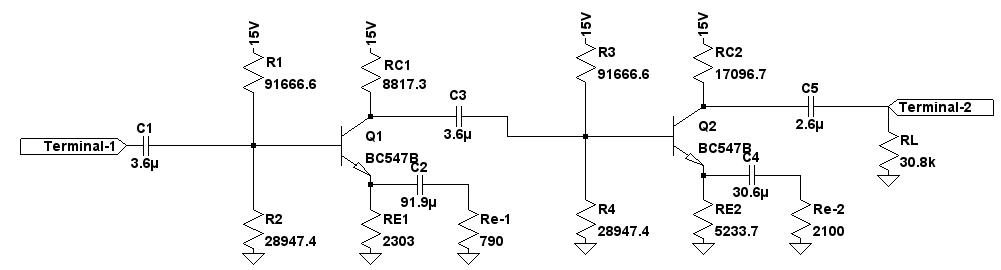
\includegraphics[scale=0.42]{maalerapporter/forforstaerker/testobjekt-forforstaerker.png}
\caption{Forforstærker med angivelser af terminaler}
\label{fig:testob_efforstaerker}
\end{figure}

\subsection*{Måleopstilling}
Målingerne foretages med to forskellige opstillinger; én til impedansmåling og én til forstærkning-, frekvensgang- og forvrængningsmåling. Opstillingerne er vist på figur \ref{fig:maaleop-imp} og figur \ref{fig:maaleop-thd}\fixme{kilde: Ole Kiel Jensen, mm5 maaleteknik}.

\begin{figure}[h]
\centering
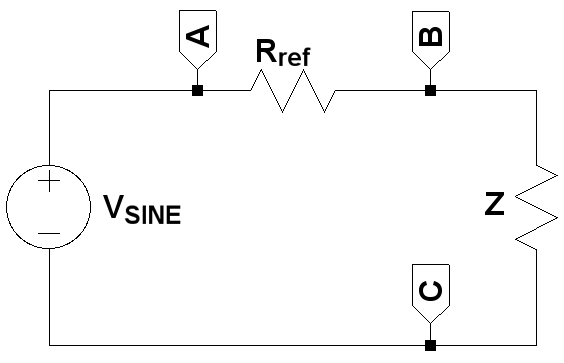
\includegraphics[scale=0.25]{maalerapporter/forforstaerker/impedansopstilling-forforstaerker.png}
\caption{Måleopstilling for impedansmåling}
\label{fig:maaleop-imp}
\end{figure}

\begin{figure}[h]
\centering
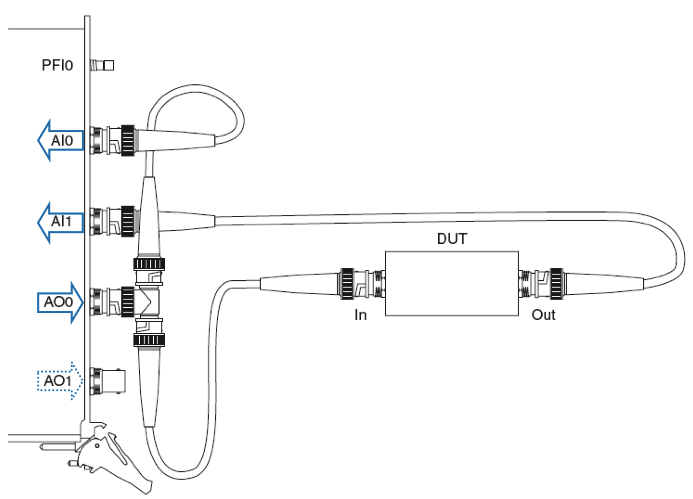
\includegraphics[scale=0.3]{maalerapporter/forforstaerker/maaleopstilling-thd-forforstaerker.png}
\caption{Måleopstilling for forstærkning-, frekvensgang- og forvrængningsmåling}
\label{fig:maaleop-thd}
\end{figure}

\subsection*{Anvendt udstyr}

RC-oscillator - AUC07997
Oscilloscope - AUC33851
Hameg triple powersupply - AUC33907
Effektmodstand 8,2 \ohm 18 Watt - AUC2159-02 B1-101-R-5
Texas instruments NI-4461 audioanalysator
Fluke - AUC08518
Fluke - AUC33048

\subsection*{Måleprocedure}

Ændringer i swept sine program
Samplingfrekvens: 204800 Hz
AI response range: +-31,6 V
AI stimulus range: +-3,16 V
Stimulus amplitude: 200 mV og 2 V
Startfrekvens: 10 Hz
Slutfrekvens: 92 kHz
THD units: \%

\subsection*{Resultater}
THD og frekvensgang blev målt for effektforstærkeren, resultaterne kan aflæses i figur \ref{fig:apeff:frek200mv} til figur \ref{fig:apeff:thd200mv} 

\begin{figure}[h]
\centering
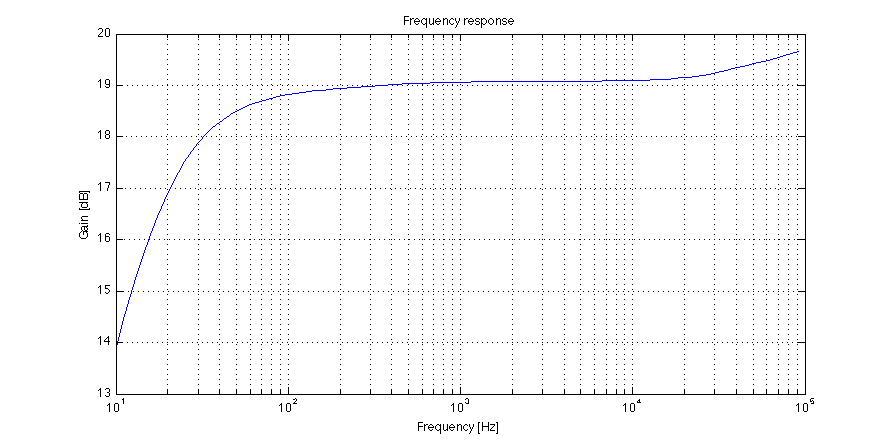
\includegraphics[width=\textwidth]{maalerapporter/effektforstaerker/200mV-45mA-uden-modstand frek.png}
\caption{Frekvensgangen for effektforstærkeren ved 200 mV.}
\label{fig:apeff:frek200mv}
\end{figure}

\begin{figure}[h]
\centering
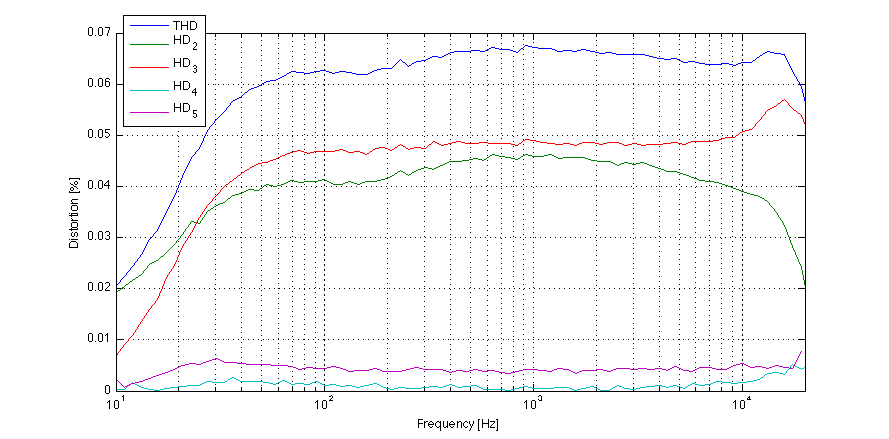
\includegraphics[width=\textwidth]{maalerapporter/effektforstaerker/200mV-45mA-uden-modstand thd.png}
\caption{THD for effektforstærkeren ved 200 mV.}
\label{fig:apeff:thd200mv}
\end{figure}

\begin{figure}[h]
\centering
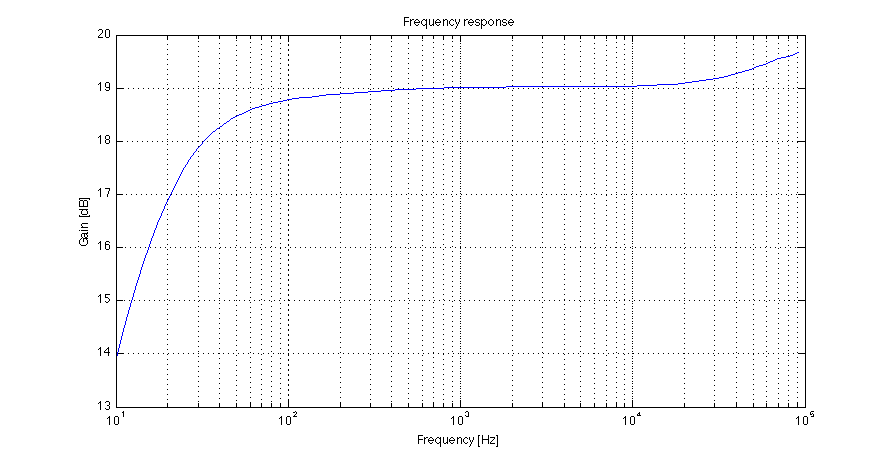
\includegraphics[width=\textwidth]{maalerapporter/effektforstaerker/2V-45mA-uden-modstand frek.png}
\caption{Frekvensgangen for effektforstærkeren ved 2 V.}
\label{fig:apeff:frek2v}
\end{figure}

\begin{figure}[h]
\centering
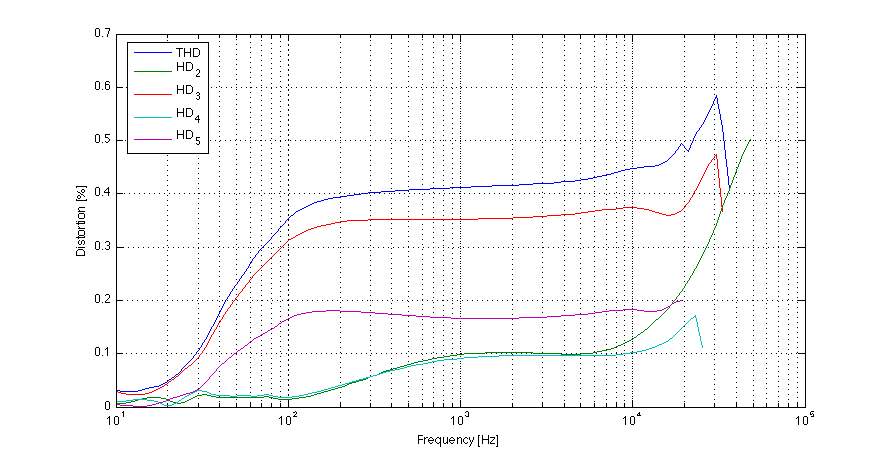
\includegraphics[width=\textwidth]{maalerapporter/effektforstaerker/2V-45mA-uden-modstand thd.png}
\caption{THD for effektforstærkeren ved 2 V.}
\label{fig:apeff:thd2v}
\end{figure}

\subsection*{Måleusikkerheder}
De væsentligste usikkerheder er:
\begin{itemize}
\item Komponent tolerancer
\item Påvirkning fra måleinstrument
\item Måleinstrument unøjagtighed
\item Støj, 50 Hz brum
\item Anden indstråling
\end{itemize}
\fixme{Kig på de her fejlkilder, i alle målerapporter}